\newpage
\section{Model Identification}

Model-based methods for controlling the arm as a unified system and determining real-world arm dynamics have been suggested in earlier studies as a solution for precise control. For instance, physics-based models have demonstrated some success in controlling two muscles for rehabilitation \cite{IOL}. However, a major challenge lies in the identification of the physical parameters of the entire arm, which demands a significant amount of data.

To address this issue, black-box model-based control methods have been developed. An example of these methods successfully utilized an artificial neural network (ANN) to create a map of task space configuration in relation to the forces that muscles can generate, thereby achieving control of planar arm tasks \cite{FC2D}. Moreover, Lyapunov-based methods have been employed to create a data-driven Deep Neural Network (DNN) based adaptive control method used for Functional Electrical Stimulation (FES)-induced leg extension rehabilitation \cite{CLDNN}.

Another difficulty lies in establishing control parameters for these systems, with new parameters needing to be set for each subject. Even for the same subject, these parameters can vary under different conditions, making the traditional control theory that requires a mathematical model of the controlled system unsuitable \cite{NNPID}. 

Despite the potential of model-based FES control in providing necessary accuracy, few approaches have found their way into clinical practice. This shortfall can be attributed to challenges in deriving an accurate model given the limited identification time due to factors such as onset of fatigue and time constraints of the patient, carer, physiotherapist, or engineer \cite{IOL}. Furthermore, due to time-varying physiological effects, models must be re-identified at the commencement of each treatment session.

Previous work has demonstrated that a semi-parametric Gaussian Process Regression (GPR) model can form the foundation for a controller achieving three-dimensional dynamic trajectories. This model-based method \cite{QSC} circumvents parametric modelling challenges owing to the difficulty in defining the parameters. The semiparametric GPR combines the generalization potential of a parameterized model with the ability of a nonlinear function approximator that represents the diversity of the musculoskeletal dynamics. 

In this project, we developed our model identification in a manner akin to the approach outlined in the paper \cite{QSC}, as it was found to be successful in circumventing the challenges intrinsic to parametric modeling. The GPR model provides a non-parametric, data-driven approach, allowing for an analytical representation of complex patterns without necessitating rigid assumptions regarding the model's structure.

\subsection{Design}

 A two part modeled is developed consisting of:

 \begin{itemize}
     \item \textbf{Inverse Statics}. It calculates the joint torque needed to hold a desired static arm configuration.
     \item \textbf{Muscle Torque Production}. It maps the arm configuration with the muscle activation to the joint torque produced by this activation and the specific arm configuration. 
 \end{itemize}

To gather data for the models a PI controller is designed to compute the force applied at the wrist in order to hold the arm in a static position, both with and without neural excitation. This force is subsequently converted into torque using the kinematic Jacobian. The process is detailed in the following sections. 

 \subsection{Target Positions and Initial Configuration}

 In the paper \cite{QSC} the simulated experiment resembles the one performed in a real-case scenario. A total of 27 different positions were analyzed where an external robot held the wrist of the arm into the different static positions. The robot was equipped with a three-dimensional force sensor at its end-effector \cite{HSAC}. 
 
 Since no real-world situation has been evaluated for this project, the simulation's goal is to represent a reaching motion beginning from an equilibrium posture. Additionally, the stroke survivor's arm is not being held by an external robot.As detailed in Section X, this approach stems from the assumption that the stroke survivor retains a degree of arm stability, sufficient to facilitate a limited reaching movement.  

 For this, it is decided to find calculate the forces in 64 different positions. This 64 positions are automatically generated using the function \textit{\textbf{create\_grid()}}.


The \textbf{\textit{create\_grid()}} function generates a grid of target points by defining the starting and ending coordinates for the x, y, and z dimensions and then linearly spacing these coordinates. If a model is provided as an input, the function also plots the wrist references, offering a visual representation of these coordinates.

\begin{table}[h]
    \centering
    \caption{Start and End Positions for x, y, and z Coordinates}

    \begin{tabular}{|c|c|c|}
        \hline
        Coordinate & Start Position & End Position \\
        \hline
        x & 0.3 & -0.08 \\
        y & 0 & -0.3 \\
        z & -0.1 & -0.35 \\
        \hline
    \end{tabular}
    \label{table:coordinates}
\end{table}

\begin{figure}[h!]
    \centering
    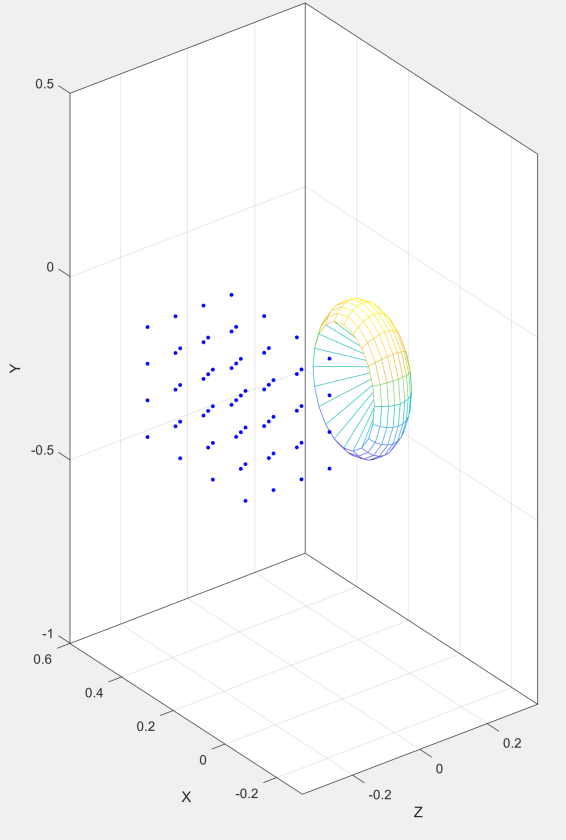
\includegraphics[width=0.4\textwidth]{Pictures/Model/create_grid.png}
    \caption{\textit{create\_grid} function output. 64 target positions used to calculate the required force to hold a this reference static positions with and without neural excitation.}
    \label{fig:create_grid}
\end{figure}

\newpage
\subsection{PI Force Controller}

 The goal of the static force simulation is to determine the necessary force to keep the wrist in a specific static position. It involves two distinct scenarios. Both scenarios use a PI controller to exert the required force at the wrist, using the input \textit{handF} in the \textbf{\textit{das3\_step(...)}} function (refer to Equation \ref{matlab:das3step}).

\begin{figure}[h!]
    \centering
    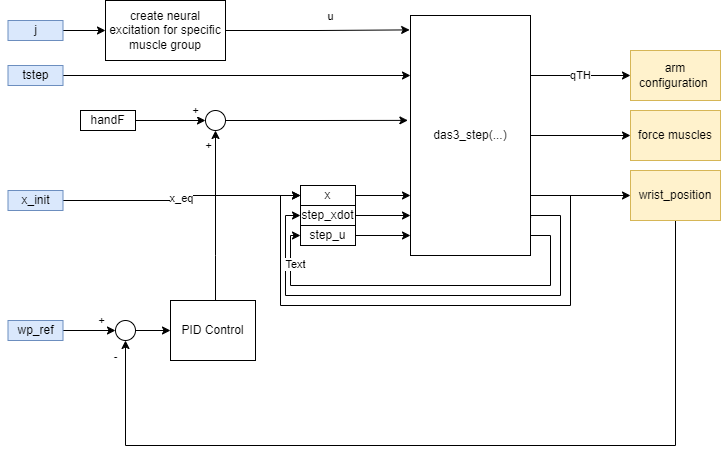
\includegraphics[width=0.9\textwidth]{Pictures/Model/PIController.png}
    \caption{Block Diagram for PI Force Controller}
    \label{fig:PIBlockDiagram}
\end{figure}

In the first scenario, no muscles are excited. The simulation starts from the equilibrium position and continues for 3 seconds, with a time step of 0.001 seconds. The focus is to calculate how much force is needed to apply to maintain a specific arm configuration static.

In the second scenario, the simulation begins with the arm configuration that was determined after running the previous no-excitation simulation. Here, one muscle at a time is stimulated at 100\%, i.e, $u_{j}$. The index j represents the muscle, this values goes from 1 to 9. Although the muscles may deviate from the starting position, the PI controller continuously adjusts to keep the hand in its initial position. This simulation is shorter, running for 0.5 seconds, but still utilizes a time step of 0.001 seconds.

After each time step,in both scenarios, the difference between the wrist's current position and the target is computed. This error is then multiplied by the Proportional (P) coefficient (Kp) of the PI controller. Concurrently, the accumulated error is updated and multiplied by the Integral (I) coefficient (Ki).  The sum of both the proportional and integral terms dictates the \textit{handF} for the next step. In the context of the PI controller, the Proportional segment is responsible for creating an output in direct relation to the present error, while the Integral portion systematically reduces  steady-state error by considering the history of past errors.

The specific values for T, $t_{step}$, PI parameters for both scenarios are detailed in Table \ref{tab:PI}.

The force necessary to reach each point is calculated by averaging the last 10\% of the data collected during the simulation.The resulting information, including the forces exerted, mean force, and the arm's configuration, is  saved for each point in the simulation.

\begin{table}[h]
    \centering
    \caption{Values for Period (T), Time step ($t_step$), and PI Gains for PI controller with no neural excitation ($u_j=0$) and with neural excitation for each muscle ($u_j = 1$). The index j represents each muscle $j \epsilon[1,9]$.}
    \begin{tabular}{|l|c|c|}
        \hline
        \textbf{Parameter} & \textbf{$u_j=0$} & \textbf{$u_j=1$} \\
        \(T\) (Period) & 3 & 0.5 \\
        \(t_{step}\) (Time Step) & 0.001 & 0.001 \\
        \( K_p \) (Proportional Gain) & 2000 & 2000\\
        \( K_i \) (Integral Gain)     & 100 & 100 \\
        \hline
    \end{tabular}

    \label{tab:PI}
\end{table}

\newpage
Below is a MATLAB code snippet that demonstrates the calculation of PI force, inclusive of the step simulation.

\begin{lstlisting}[style=Matlab-editor]
hand_current = wrist_position(x)
error_pos = hand_goal - hand_current
error_int = error_int + error_pos*tstep;

% PI calculation for time step
handF = K*error_pos+I*error_int;

[x, xdot, step_u] = das3step(x, u, tstep, xdot, step_u, M, exF, handF);
\end{lstlisting}

The function \textbf{\textit{wrist\_position(x)}} calculates the global position of the wrist using transformation techniques. Initially, the \textit{das3('Visualization',..)} is wrist position vector ($p$) and the orientation matrix ($R$). Constants and position vectors are defined, including the local coordinates of bone points.

Next, the function transforms the local coordinates into global ones. By utilizing the orientation matrix $\textbf{R}$ and the position vector $\textbf{p}$, it applies a transformation to the local coordinates, yielding the global coordinates \textbf{x}, \textbf{y}, and \textbf{z}. The process is a straightforward application of the principles of rotation and translation, aligning the local wrist coordinates with a global frame of reference.

\begin{equation}
\begin{aligned}
    p_{rotated} = R*p_{local} \\
    p_{global} = p_{rotated} + t
\end{aligned}
\end{equation}

where $p_{rotated}$ is the rotated position vector, $R$ is the orientation matrix, $p_{local}$ is the local position vector, and $t$ is the translation vector representing the shift from the local to the global coordinate system.


\newpage
\subsection{Kinematic Jacobian and Torque Calculation}

The Kinematic Jacobian is a critical part of the transformation of the recorded robot controller force to the joint torque $\tau_j$. The index j represents the muscle group being activated, when no muscle is being activated j is equal to 0.

In robotics, the Jacobian matrix provides essential information about the relationship between the velocities of the joints and the end-effector of a robot manipulator. This relationship can be expressed using the equation

\begin{equation}
\dot{x} = J \cdot \dot{q}
\end{equation}

where $\dot{x}$ is the end-effector velocity and $\dot{q}$ is the joint velocity.

Understanding the relationship between how the robot joint's velocities correlate to the end-effector's velocities is vital for planning trajectories in different spaces.

Furthermore, the kinematic Jacobian can be use to determined the necessary forces in joint space to achieve specific forces in end-effector space. In the musculosketal system it is assumed that the 11 degrees-of-freedom have no friction at the joint. The joint torques ($ \tau \epsilon R^n$) required to bear an endpoint/hand force ($F \epsilon R^{6x1}$), are given by,

\begin{equation}
    \tau = J^T*F
\end{equation}

where the Jacobian matrix ($J \epsilon R^{6xn}$) relates the infinitesimal joint displacement $dq$ to the infinitesimal end-effector displacements $dp$. The theorem is proven using the Principle of Virtual Work \cite{ITR}.

\begin{equation}
    dq = J*dp
\end{equation} \label{eq:displacement}

This equation is applied as shown in the MATLAB code below to calculate the torque values from the mean forces previously calculate using the PI controller. 

\begin{lstlisting} [style=Matlab-editor]
[dPhand_dx, ~, ~] = handpos_jacobian(x);
torque = dPhand_dx'*hand_F;
\end{lstlisting}

Calculating the kinematic Jacobian in robotics involves defining the structure and parameters of the robot's joints and links, often using conventions like Denavit-Hartenberg (D-H) parameters. Transformation matrices are found for each joint, and the end-effector position is obtained by multiplying these matrices.

The Jacobian matrix is then constructed by differentiating the end-effector's position with respect to each joint variable, considering whether the joint is revolute or prismatic. The resulting 6×n matrix, where n is the number of joints, maps the joint velocities to the linear and angular velocities of the end-effector.

Due to the complex system, to calculate the kinematic Jacobian the concept of infinitesimal displacement presented in Equation \ref{eq:displacement} is used. The function \textbf{\textit{handpos\_jacobian(x)}} (MATLAB code below) take the state and perturbs each degree of freedom by a small mount $h$. For each perturbation, the old and the new hand positions are  subtracted and divided by $h$. This describes how the changes in the degrees of freedom affect the hand´s position at that particular state. 

\begin{lstlisting}[style=Matlab-editor]
function [dPhand_dx, Phand, Phand_new] = handpos_jacobian(x)
    dPhand_dx = zeros(3,11);
    stick = das3('Visualization', x);
    Phand = stick(13,1:3)';
    h = 1e-7;
    for i = 1:11
        tmp = x(i);
        x(i) = x(i) + h;
        stick = das3('Visualization',x);
        Phand_new = stick(13,1:3)';
        dPhand_dx(:,i) = (Phand_new - Phand)/h;
        x(i) = tmp;
    end        
end
\end{lstlisting}

The shoulder and elbow torques are computed using the transpose of the kinematic Jacobian. They are denoted by $\tau_{j}$, where $j$ symbolizes the muscle group being activated, with 0 signifying no active muscles. The torque concerning elbow pronation is disregarded as it does not influence the wrist's positions. 

If no muscles are activated, the torque needed to hold the the wrist in static position is equal to,

\begin{equation}
\tau_0 = p(q)
\end{equation}

where $p(q) \epsilon  R^{4x1}$. 

The torque produced by the muscle's group $j$ activations is calculating by subtracting the torques recorded when no muscles are activated and the torques recorded with muscle group $j$ active. This torque  is represented by $R(q)\alpha$ where $\alpha \epsilon R^{9x1}$ is the vector of muscle group activations and $R(q) \epsilon R^{4x9}$ is the mapping from muscle group activation to joint torque. It is assumed that the torques scales linearly with activation \cite{SPI}. 

\begin{equation}
    R_j(q) = \tau_0 - \tau_j
\end{equation}

Each column of $R(q)$ describes the torque generated by each muscle group at full activation. It is assumed that individual muscle torques add linearly without interference from adjacent muscles or connective tissue interactions. 





\subsection{Gaussian Process Regression}